\documentclass{article}

\title{Graphics P1 Usage}
\date{10/03/2019}
\author{150008859}

\setlength{\parskip}{1em}
\setlength{\parindent}{0em}

\usepackage{listings}
\usepackage{amsmath,amssymb,amsthm}
\usepackage{mathtools}
\usepackage{graphicx}
\usepackage{subfig}
\usepackage{xcolor}

\begin{document}
\maketitle

\section{2d Tool}

Run the 2d tool by entering the practical directory and running:

\begin{verbatim}
java -cp bin draw.BezierDraw2d
\end{verbatim}

\subsection{Control Points}

\begin{table}[ht!]
  \centering
\begin{tabular}{||c c||}
  \hline
  Input & Description \\
  \hline \hline
  Left Click & Insert a new Point  \\
  \hline
  Scroll Wheel Click & Drag to move a Control Point  \\
  \hline
  Right Click & Delete a Point  \\
  \hline
\end{tabular}
\end{table}

\begin{figure}[!htb]
  \caption{Inserting Control Points. }
  \centering
  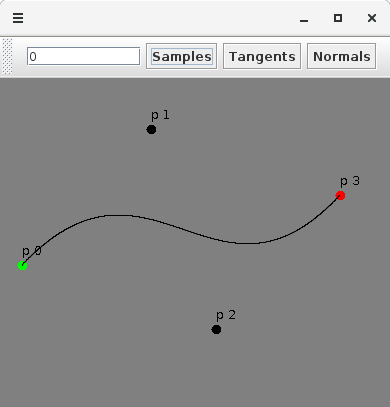
\includegraphics[scale=0.38]{images/image1.png}
\end{figure}

\subsection{Tangents and Curvature Normals}

After inserting some control points, specify number of sample points and press ``Samples''.

Click Tangents and Normals to toggle them on or off.

Tangents in blue and normals in pink.

\begin{figure}[!htb]
  \caption{Tangents and Curvature Normals. }
  \centering
  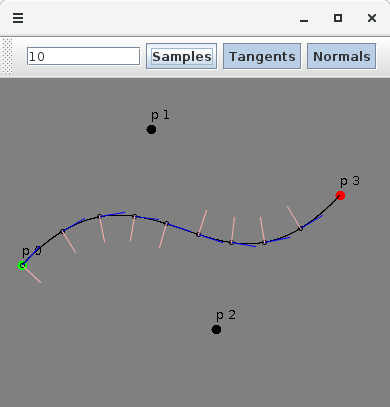
\includegraphics[scale=0.38]{images/image2.png}
\end{figure}

\section{3d Tool}

Run the 3d tool by entering the practical directory and running:

\begin{verbatim}
java -cp bin draw.BezierDraw3d
\end{verbatim}

\subsection{Generate a Curve or Surface}

\begin{figure}[!htb]
  \caption{Specify n and click Curve to draw a Bezier Curve.}
  \centering
  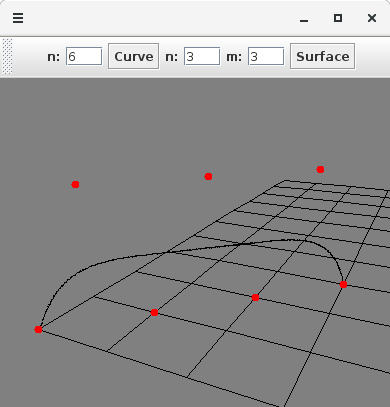
\includegraphics[scale=0.38]{images/image3.png}
\end{figure}

\begin{figure}[!htb]
  \caption{Specify n, m and click Surface to draw a Bezier Surface.}
  \centering
  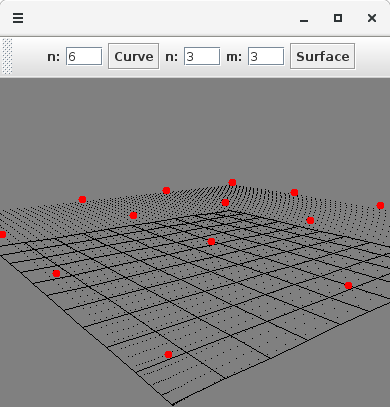
\includegraphics[scale=0.38]{images/image4.png}
\end{figure}

\subsection{Camera}

Reposition Camera using WASD.

\begin{table}[ht!]
  \centering
  \begin{tabular}{||c c||}
    \hline
    Input & Description \\
    \hline
    \hline
    W & Move Forward \\
    \hline
    A & Strafe Left  \\
    \hline
    S & Move Back \\
    \hline
    D & Strafe Right \\
    \hline
  \end{tabular}
\end{table}

Look around using the Arrow Keys.

\begin{table}[ht!]
  \centering
  \begin{tabular}{||c c||}
    \hline
    Input & Description \\
    \hline
    \hline
    $\uparrow$ & Look Up \\
    \hline
    $\downarrow$ & Look Down \\
    \hline
    $\leftarrow$ & Look Left  \\
    \hline
    $\rightarrow$ & Look Right \\
    \hline
  \end{tabular}
\end{table}

\subsection{Edit Control Point}

\begin{figure}[!htb]
  \caption{Select a Control Point by clicking on it, edit control point using WASD and RF for elevation. }
  \centering
  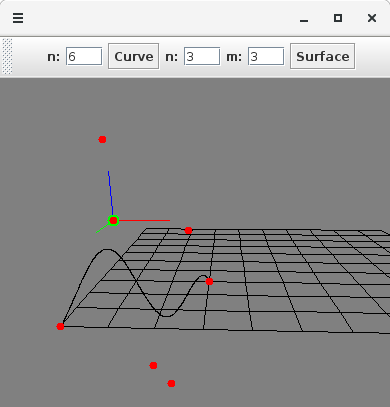
\includegraphics[scale=0.38]{images/image5.png}
\end{figure}

Movement along z axis (green).

\begin{table}[ht!]
  \centering
  \begin{tabular}{||c c||}
    \hline
    Input & Description \\
    \hline
    \hline
    W & $-$ Movement along z axis  \\
    \hline
    S & $+$ Movement along z axis \\
    \hline
  \end{tabular}
\end{table}

Movement Along x axis (red). 

\begin{table}[ht!]
  \centering
  \begin{tabular}{||c c||}
    \hline
    Input & Description \\
    \hline
    \hline
    A &  $-$ Movement along x axis \\
    \hline
    D &  $+$ Movement along x axis \\
    \hline
  \end{tabular}
\end{table}

Elevation (blue).

\begin{table}[ht!]
  \centering
  \begin{tabular}{||c c||}
    \hline
    Input & Description \\
    \hline
    \hline
    R & $+$ Movement along y axis \\
    \hline
    F & $-$ Movement along y axis \\
    \hline
  \end{tabular}
\end{table}

\begin{figure}[!htb]
  \caption{A cool Bezier Surface.}
  \centering
  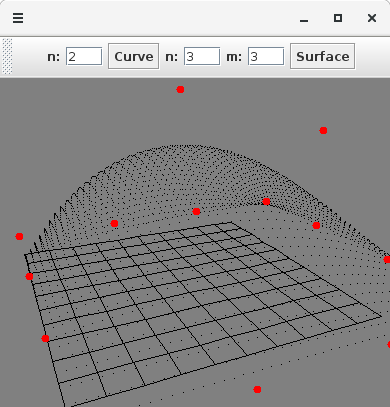
\includegraphics[scale=0.38]{images/image6.png}
\end{figure}



\end{document}
